\section{Frozen global-search evidence}\label{sec:evidence45}
\subsection{Design, information, and computational accounting}
The global experiment consists of twelve designed cases from three families and four variants of a separate near-tie construction. Within each primary family, $(n,T,m)$ takes values $(4,4,3)$, $(8,8,3)$, $(8,16,4)$, and $(16,32,4)$. The corresponding $(\beta,\varepsilon)$ pairs are $(0.9,0.01)$, $(0.95,0.01)$, $(0.95,0.005)$, and $(0.95,0.001)$. Every method receives identical rational rewards, costs, controlled transition probabilities, initial law, and restart inequalities. The inventory and queueing primitives use discrete demand or arrival shocks; the maintenance family varies controlled regime transitions. The exact generators are specified in the supplement.

The final source freeze precedes these executions and includes eleven scientific source hashes and sixteen primitive hashes. The registered allowance is 120 seconds and 2,047 nodes per method, with 15 seconds per node LP and at most five seconds for a local root proposal. A budget check occurs between proof-producing node operations: an iteration can exceed the nominal wall cap while completing a valid node or its sibling. Measured time, rather than the nominal cap, is reported. Exact checking time is charged separately. Every method was run with one numerical thread; the environment records Python 3.13.15, NumPy 2.3.5, SciPy 1.17.0, and PySCIPOpt 6.2.1 on a four-CPU Linux runner. Paired methods in a case use the same runner. Hardware equivalence is not inferred across separately scheduled cases.

Method B uses Bellman supports, disaggregated products, and simplex-product consistency. Method A uses the aggregate-product relaxation. Both use the same common-policy repair and covering-tree contract. A local nonlinear optimizer can propose a root candidate, but its output is quantized and repaired before it affects an upper endpoint. Every node also evaluates its lower-corner policy. Thus soundness and theoretical completeness do not depend on success of the local optimizer or on a favorable LP proposal.

SCIP uses the common-policy bilinear equations, the same root domains, Bellman supports, and strict-gap cones when applicable. Its objective, feasibility tolerance, random seed, one-thread setting, absolute-gap target, and budgets are recorded. This grants the external solver the same strengthening information rather than withholding the method's cuts. Its native lower endpoint is a floating-point solver assertion; its proposed policy is independently evaluated after rational repair. No claim is made that SCIP cannot provide other verification modes. The comparison concerns this executed nonlinear adapter.

\subsection{Every global interval, including unsuccessful stops}
\begin{table}[t]
\caption{All frozen global cases: absolute widths at target $10^{-3}$}\label{tab:global45}
\centering\small\setlength{\tabcolsep}{4pt}
\begin{tabular}{lrrr rrr l}\toprule
Case&$n$&$T$&$m$&B width&A width&Intersection&Target met\\\midrule
\tablerows{revisions/2026-09-25-r45/paper/generated/global_summary.tex}
\bottomrule\end{tabular}
\par\smallskip\footnotesize M: maintenance; I: inventory; Q: queueing; T: near-tie variants. B and A are independently checked whole-tree intervals, not root LP statuses. The intersection uses the largest checked lower endpoint and the smallest checked feasible upper cost, including SCIP's repaired candidate. It combines separate computations and is not a single 120-second algorithm. Target tests use exact fractions, not rounded displays. Full endpoints, relative widths, work, and stop reasons are in the supplement.
\end{table}
Table~\ref{tab:global45} keeps all sixteen cases. B has narrower final intervals in eleven cases, A in four, and one pair is equal. Nevertheless B meets the target in four cases and A in five. Their certified intersection, including the independently evaluated SCIP policy, meets it in five. A narrower root bound or a larger formulation is not enough to predict final target attainment under a fixed budget.

There is now successful closure after branching. On Q1, B reduces its gap below $10^{-3}$ in 49 nodes; A requires 153 nodes. On M0, A closes in 13 nodes, whereas B already closes at its root. I0 is a zero-cost case, and Q0 is nearly exact at the root; they are not counted as demonstrations of difficult search. Q3, the largest queueing case, closes under A at the root. B explores only seven nodes and leaves a width about $0.0322$ there. All three largest cases favor A's final width. Proof construction and stronger per-node relaxations consume resources that otherwise support further branching.

\begin{figure}[t]\centering
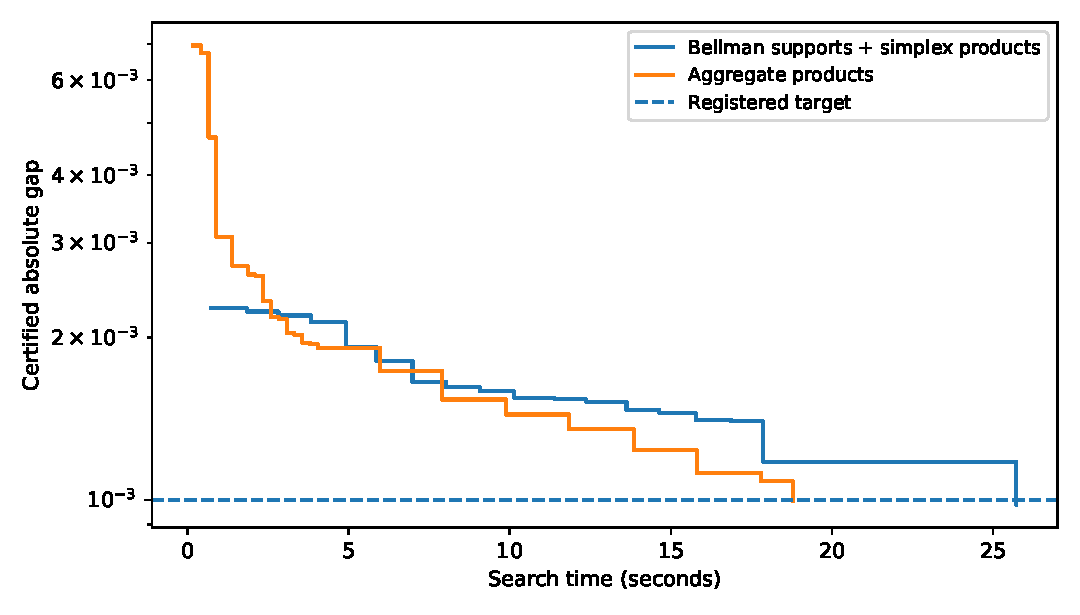
\includegraphics[width=.9\linewidth]{revisions/2026-09-25-r45/paper/generated/queue1_progress.pdf}
\caption{Certified gap along the recorded Q1 searches. Every plotted point is an archived full-cover lower endpoint paired with the current feasible incumbent. Time excludes the final independent checker, whose cost is reported separately. The horizontal line is the registered absolute target.}\label{fig:progress45}
\end{figure}

\begin{table}[t]\caption{External global baseline: numerical gaps and verified intersections}\label{tab:scip45}
\centering\small\setlength{\tabcolsep}{4pt}
\begin{tabular}{llrrrr}\toprule
Case&SCIP stop&Native width&Nodes&Seconds&Checked intersection\\\midrule
\tablerows{revisions/2026-09-25-r45/paper/generated/native_baseline.tex}
\bottomrule\end{tabular}
\par\smallskip\footnotesize Native widths use SCIP's floating-point primal and dual bounds; they are not independent lower certificates. The final column has the same certified construction as Table~\ref{tab:global45}. Native run time includes model construction and candidate repair; independent candidate checking and the two custom lower-bound computations are not hidden inside that time.
\end{table}
SCIP reports eight native target hits. It often returns smaller numerical gaps substantially faster than the custom proof-producing search. Its failures, including node limits on inventory and tie cases and time limits on the largest maintenance and inventory cases, are also retained. This evidence does not establish computational superiority of the new cuts or implementation over a modern external global solver. What the custom method adds in the reported comparison is a replayable rational covering certificate. Both the cost of that certificate and the stronger external numerical performance are visible.

\subsection{Exact and near operating ties}\label{sec:ties45}
The tie model has four states, eight periods, three actions, $\beta=0.95$, and $\varepsilon=0.01$. The first two operating rewards are $0$ and $-\tau$, while the third is $-1/5-i/40$; terminal operating reward is zero. Actions induce different transitions. Their implementation costs are respectively $1+i/4$, $7/10+i/8$, and zero. The four values of $\tau$ are $0$, $10^{-8}$, $10^{-4}$, and $10^{-2}$. Thus $\tau=0$ is an exact operating tie with distinct implementation costs and transitions, not two duplicated actions.

B's final widths in these four cases are approximately $0.004995$, $0.005256$, $0.003211$, and $0.134494$. A's corresponding widths are $0.160574$, $0.200032$, $0.167849$, and $1.360331$. All four remain above target, even though the support formulation substantially improves the intervals. The rational validity tests succeed at $\tau=0$. This demonstrates validity and useful tightening near indifference, not target-level tie closure. The gap-free theorem explains why a positive operating gap is unnecessary for eventual finite-model certification; the observed budgets remain a separate constraint.

\subsection{Allowance scaling and the exact-LP distinction}\label{sec:scaling45}
A further frozen calculation uses one $n=3,T=8,m=3$ model from each primary family, seven allowances from $10^{-1}$ to $10^{-7}$, and both earlier root relaxations: 42 root outputs, not 42 independent environments. Each output has its own rational certificate. The complete tables report measured widths, width divided by $\varepsilon^2$, $\overline E_D$, $E_{S,0}$, $D_C$, $\chi$, the repair fraction, and the sufficient exact-LP bound \eqref{eq:quadratic45}.

The maintenance scaled widths at allowances $10^{-3},10^{-4},10^{-5}$ are approximately $0.0140484$, $1.44063\times10^{-4}$, and $1.44446\times10^{-6}$. Their ratios to $\varepsilon^2$ are close to $1.4\times10^4$ over that range. At $10^{-6}$ and $10^{-7}$ the ratios increase, so the finite-precision output is not assigned a universal quadratic exponent. The inventory model contains ties; the strict-gap bound does not apply, and its scaled and unscaled widths coincide. Queueing widths reach roughly $10^{-10}$ over several allowances, making a log--log slope a description of numerical residuals rather than the theoretical rate. The unscaled queueing run at $10^{-6}$ returns a width about $5.3153$ and is retained.

The theorem's clean bound and the realized interval measure different quantities. The available artifacts do not certify an optimizing primal--dual pair for every numerical root relaxation separately from the deployment repair. Therefore an exact numerical LP-optimality-loss decomposition is marked unavailable, not filled with zeros from an ``optimal'' status. The full measured rational interval is nevertheless valid. The former four-point scaling calculation and all eight earlier controlled root pairs are retained; none of those eight earlier environments met the $10^{-3}$ absolute target, and two returned uninformative $[0,U]$ intervals under both relaxations.

\section{Economic interpretation and the retained continuous-state evidence}\label{sec:old45}
The original maintenance state is $x\in[0,1]$, with three actions and shock probabilities $3/5,2/5$. Discounting is $19/20$, the stage operating reward is $x-c_a$ for $c=(0,3/20,9/20)$, terminal payoff is $x/2$, and revision weight is $1+x$. The two successors under each action are
\[
 (3x/4,3x/4+1/20),\quad
 (17x/20+1/10,17x/20+7/50),\quad
 (x/10+4/5,x/10+17/20).
\]
These are controlled continuous-state atoms. The primary cohort uses seven installed rules, horizons $4,8,12$, allowances $0.01,0.05$, and the uniform initial law. The forty-two configurations are a development cohort, not independent observations. All their endpoints and alternative initial-law calculations are preserved.

\begin{table}[t]\caption{Original primary cohort: open intervals and strict policy-class savings}\label{tab:primary45}
\centering\small
\begin{tabular}{rrrrrrr}\toprule
$T$&Positive&Median width (\%)&Max. (\%)&Strict gains&Min. gain&Max. gain\\\midrule
\tablerows{revisions/2026-09-25-r43/paper/generated/primary_gap_savings.tex}
\bottomrule\end{tabular}
\par\smallskip\footnotesize Width is $(U_R-L_R)/U_R$ among positive-cost randomized intervals. A strict gain is $L_D-U_R>0$, with $L_D$ a deterministic lower bound and $U_R$ a feasible randomized cost. Gain extrema condition on positive gains. The twelve zero-cost configurations are not included in the width statistics. These are retained certificates, not newly optimized rows.
\end{table}
All thirty positive-cost randomized intervals remain open. Their median relative widths increase from $5.24\%$ at horizon four to $14.33\%$ at horizon eight and $15.75\%$ at horizon twelve. Twenty-seven randomized upper policies nevertheless lie strictly below deterministic lower bounds. These two statements are compatible: a policy-class separation does not identify the randomized optimum. The finite frozen cohort is not a replacement for closing these controlled continuous-state intervals.

\subsection{Randomization as an institutional choice}
The admissible lottery is a fresh state-dependent action draw at each date, with realized departure charged under $k_t$. Suppose an organization additionally charges $f\ge0$ per use of a nondegenerate lottery. For a certified policy $p$, let
\[
 B(p)=\E_\nu^p\sum_{t=0}^{T-1}\beta^t\ind\{p_t(\cdot\mid X_t)\text{ is nondegenerate}\}.
\]
If $s=L_D-U_R>0$, the same deployed policy remains strictly cheaper than every feasible deterministic rule whenever $fB(p)<s$. A conservative sufficient condition is $f\Ssum T<s$. A one-time fixed governance cost $F$ instead requires $F<s$. This is a break-even implication in the model's implementation units, not an estimate of actual administrative costs. Such overhead changes the economic objective and must be specified before treating the new optimum as a reported result. Deterministic lower bounds remain a valid comparator because deterministic policies pay no lottery overhead.

For reporting the scale of each separation, the relevant normalized gains are $s/L_D$ and $s/U_R$, not an operating-welfare percentage. The historical numerical sources retain the signed gains, deterministic bounds, and upper-policy costs. Any percentages computed only from rounded display tables must be labeled approximations rather than exact certificates. No empirical prevalence of feasible organizational randomization is inferred from the designed cohort.

\subsection{Other continuous-state classes and the nonlinear experiment}
The twelve exact-aggregation service examples retain their tightly closed finite-LP intervals, with atomic but economically ancillary continuous coordinates. The density-transfer exercise retains the failed sufficient tightening at its largest perturbation. The observable-fiber example retains the sixteen-cell interval $[10.074215,10.184476]$, with width contributions about $0.074982$ from finite endpoints and $0.035279$ from partition variation. Seventeen endpoint solves represent one parametric family, not seventeen model tests. No newly refined or higher-dimensional fiber computation is claimed.

The nonlinear two-state model has four actions, bilinear successors, and two shocks. At allowance $1/2$, retained relative widths at $(T,N)=(8,64)$, $(16,128)$, $(32,64)$, $(32,128)$, and $(32,256)$ are $76.01\%,45.32\%,61.05\%,35.11\%,25.13\%$. Full independent arithmetic coverage is explicitly marked in the retained tables; in particular the finest $(32,256)$ object has been independently rebuilt. That audit does not turn a $25.13\%$ interval into a near-exact result. At allowance $0.05$, the retained calculations remain lower-only because no matching upper policy is certified. A failed sufficient enclosure is not proof of policy infeasibility. This revision does not invent a per-candidate failure classification when the retained records do not provide one.

The inherited binary finite-state comparison also remains unfavorable to interval Bellman search on every difficult pair: the verified McCormick formulation gives stronger intervals there. The stopped-control derivations, economic sensitivities, deterministic frontiers, and earlier counterexamples remain in the historical volume without being counted as new completed optimization targets.

\section{Verification and implementation boundaries}\label{sec:verification45}
Three distinct claims require separate evidence. The economic and mathematical reduction must preserve \eqref{eq:target45}. The arithmetic must prove each serialized inequality. The publication must match the checked source and outputs. Hashes address identity, not theorem validity. Finite adversarial tests probe the checker, not the full space of possible bugs.

The standalone tree reader imports neither optimizer nor constructor. It independently rebuilds the model, operating value, reference, supports, product domains, dual residual bounds, policy values, and every split of the global cover. Every feasible upper is checked after every state and date. SCIP candidate checks verify only the feasible policy and its cost, not SCIP's native global lower bound. The local replication of this revision checks all 32 complete custom trees and all 16 SCIP policies against their frozen model files; the exact reports accompany the manuscript. The 42 root-scaling certificates are separately identified and checked by the earlier standalone root reader.

The frozen transformation audit checked 81 deterministic and 64 mixed policies, with 19,720 support inequalities, including an exact operating tie. Seventeen archived adversarial mutations were rejected. They include forged endpoints, invalid probabilities, dual signs, nonstochastic transitions, altered discount factors, incorrect primitive disadvantages, exchanged action labels, malformed probability/product boxes, forged repair rows, missing leaves or siblings, a coverage gap, and a cyclic tree. These are finite tests, not machine-checked proofs of the general support or stopping theorems. The theorem--code matrix records which theorem is implemented, which assumptions are analytic, and which calculations were actually executed.

The final manuscript and response introduce analytic results beyond the frozen code: the explicit multi-action numerical-floor theorem, affine approximate-tie cones, and repair-density theorem. They are accompanied by proofs and separated from the predeclared numerical claims. The frozen implementations and unfavorable outputs remain unchanged. In particular, an adaptive-precision extension and the atom-preserving upper enumeration are not described as completed numerical experiments.

The new precision contract was also checked with a separate exact-rational implementation on 256 seeded two-state, three-date, three-action boxes, including an exact operating tie. Every surviving box satisfied the ideal-repair stopping inequality and all repaired restart constraints. A separate exact implementation checked the quantized operating-reference repair on those same 256 boxes, including its rounding guard; all also satisfied the two-grid bound. These are two contract checks on the same boxes, not 512 independent test environments. Sixteen additional exact calculations report sufficient precision floors and box widths for the frozen models. These tests check instances of the mathematical contract; the proofs, not the test count, establish the theorems. All forty-two frozen scaling proof objects were independently replayed as well.

\section{Conclusion}\label{sec:conclusion45}
Minimum-cost revision under all-restart operating protection is a common-continuation problem. Backward feasibility repair provides an explicit connection between numerical approximation and admissible deployment. Bellman supports and a multi-action covering search extend this connection to operating ties, while a precision-dependent stopping modulus makes the role of finite arithmetic explicit. The strictly separated small-allowance rate is retained as a sharper conditional result, not a universal numerical law.

For controlled continuous states, the repair-density theorem keeps the unrestricted Borel policy target and permits action-dependent atoms. It supplies a convergent upper approximation; valid support witnesses supply lower bounds without atom smoothing. A matched two-sided convergence rate for the original controlled continuum remains a distinct task. Exact aggregation and observable-fiber identities continue to give paired results under their stated structure.

The complete-search evaluation now records real branching, a modern external baseline, all failed stops, and complete arithmetic covers. Five of sixteen combined rational intervals meet the registered target. The stronger custom relaxation does not dominate the cheaper one at the largest scale, and SCIP often delivers better native numerical performance. Those results identify the value and cost of independently verifiable certification. They do not erase the original thirty open positive-cost randomized intervals or the economic assumptions behind admissible randomization. The policy-class savings and the certification methods are substantive results on their stated objects, not substitutes for unperformed calibration or unsupported claims of universal tractability.
